\subsection{Dashboard}
Una \textit{dashboard}\textsubscript{\textit{G}} costituisce il cruscotto di controllo primario del \textit{sistema}\textsubscript{\textit{G}}, rappresentando una composizione di diversi pannelli che visualizzano i dati in tempo reale provenienti dai sensori. \\
Ogni pannello consente la visualizzazione dei dati in modo appropriato, adottando grafici di diversa natura in base alla tipologia di informazioni. Ad esempio, nel caso di dati temporali, il pannello mostrerà un grafico a linee, mentre per la visualizzazione di dati spaziali, sarà presentata una mappa interattiva che illustra la posizione, la tipologia e le misurazioni dei sensori.\\
Per ciascun gruppo di pannelli, saranno inclusi anche valori numerici contenenti informazioni aggiuntive e specifiche. Questi valori mostreranno aggregazioni dei dati, la disponibilità di risorse specifiche o il punteggio di salute complessivo della città. \\
\begin{figure}[H]
    \centering
    \fbox{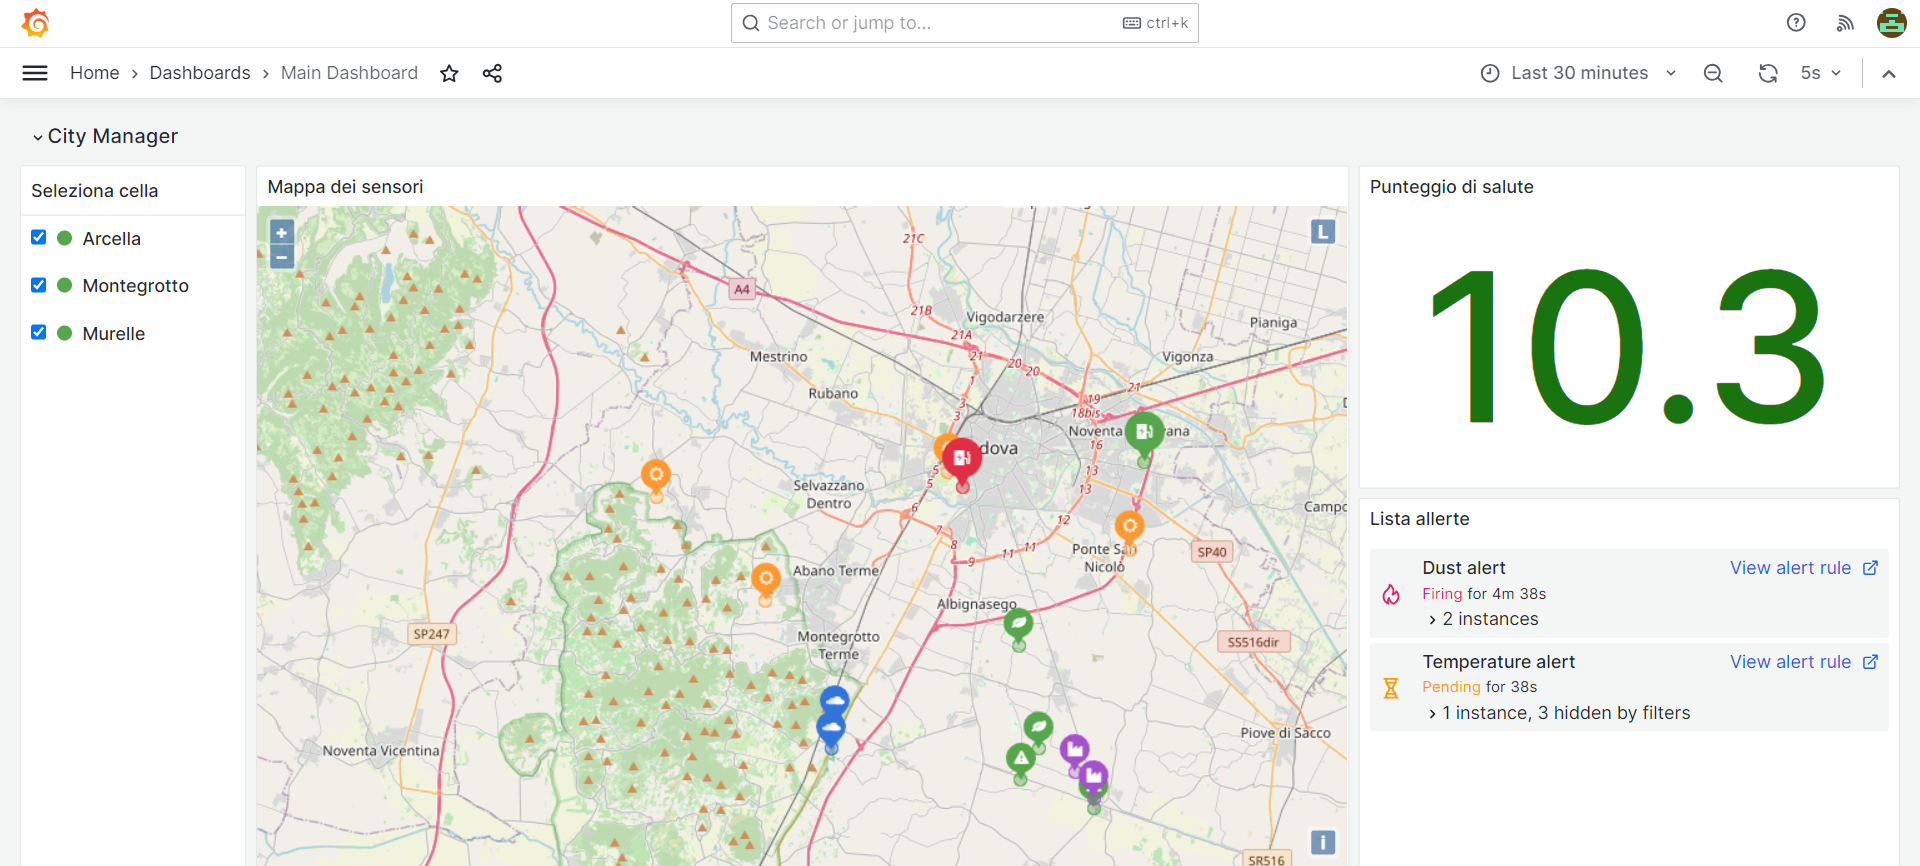
\includegraphics[width=16cm]{../Images/ManualeUtente/Light/dashboard_principale_light_alert.png}}
    \caption{Esempio di dashboard principale}
    \label{fig:my_label}
\end{figure}


\subsubsection{Barra degli strumenti}
\label{sec:barra_strumenti}
La barra degli strumenti è una sezione della \textit{dashboard}\textsubscript{\textit{G}} posizionata nella parte superiore della pagina. Essa fornisce una serie di pulsanti, icone e menu a tendina che consentono agli utenti di eseguire azioni specifiche o di accedere a funzionalità aggiuntive in modo rapido e intuitivo. \\
\begin{figure}[H]
    \centering
    \fbox{
\includegraphics[width=16cm]{../Images/ManualeUtente/Light/toolbar.png}}
    \caption{Barra degli strumenti}
    \label{fig:my_label}
\end{figure}

\paragraph{Pulsante profilo utente}
\hypertarget{par:pulsante_profilo}{}
Il pulsante del profilo utente consente all'utente di accedere al proprio profilo personale, dove potrà visualizzare e modificare le proprie informazioni personali, le impostazioni dell'\textit{account}\textsubscript{\textit{G}} e le preferenze. \\
Una volta premuto il pulsante, verrà visualizzato un menu a tendina con le seguenti opzioni:
\begin{itemize}
    \item Profile: permette di visualizzare e modificare le informazioni personali;
    \item Notification history: consente di visualizzare la cronologia delle notifiche ricevute;
    \item Change password: offre la possibilità di modificare la password dell'\textit{account}\textsubscript{\textit{G}};
    \item Sign out: permette di effettuare il \textit{logout}\textsubscript{\textit{G}} dal \textit{sistema}\textsubscript{\textit{G}}.
\end{itemize}
\begin{figure}[H]
    \centering
    \fbox{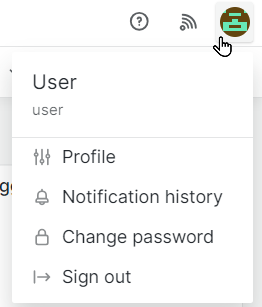
\includegraphics[width=5cm]{../Images/ManualeUtente/Light/toolbar_dettaglio_user.png}}
    \caption{Pulsante profilo utente}
    \label{fig:my_label}
\end{figure}


\paragraph{Barra di ricerca}
La barra di ricerca consente all'utente di cercare e filtrare le \textit{dashboard}\textsubscript{\textit{G}} disponibili o di cambiare pagina. L'utente può digitare il nome della \textit{dashboard}\textsubscript{\textit{G}} o della pagina desiderata e premere "Invio" per visualizzare i risultati della ricerca.  
\begin{figure}[H]
    \centering
    \fbox{
\includegraphics[width=7cm]{../Images/ManualeUtente/Light/toolbar_dettaglio_navbar.png}}
    \caption{Barra di ricerca}
    \label{fig:my_label}
\end{figure}

\paragraph{Menu ad hamburger}
Il menu ad hamburger è un'icona costituita da tre linee orizzontali sovrapposte, che rappresenta un pulsante per l'apertura di un menu a discesa. Questo menu consente all'utente di accedere a funzionalità aggiuntive. \\
Queste funzionalità sono:
\begin{itemize}
    \item Home: offre la possibilità di tornare alla homepage di \textit{Grafana}\textsubscript{\textit{G}};
    \item Starred: permette di visualizzare le \textit{dashboard}\textsubscript{\textit{G}} preferite;
    \item Dashboards: consente di accedere alla lista delle \textit{dashboard}\textsubscript{\textit{G}} disponibili;
    \item Alerting: offre la possibilità di visualizzare ed esportare le regole di allerta e notifiche;
\end{itemize}
\begin{figure}[H]
    \centering
    \fbox{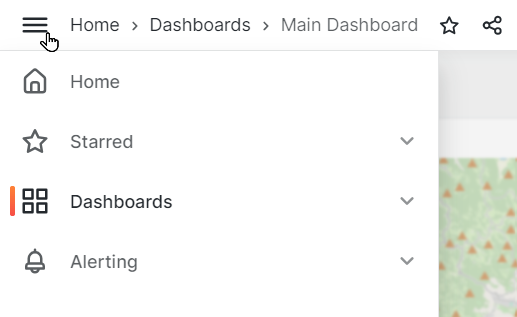
\includegraphics[width=9cm]{../Images/ManualeUtente/Light/toolbar_dettaglio_hamburger.png}}
    \caption{Menu ad hamburger}
    \label{fig:my_label}
\end{figure}

\paragraph{Breadcrumb}
Il breadcrumb è composto da una serie di \textit{link}\textsubscript{\textit{G}} che mostrano la posizione corrente dell'utente all'interno del sito. Questi \textit{link}\textsubscript{\textit{G}} consentono all'utente di navigare facilmente all'interno del sito, tornando indietro o spostandosi avanti nella gerarchia delle pagine. \\
\begin{figure}[H]
    \centering
    \fbox{
\includegraphics[width=7cm]{../Images/ManualeUtente/Light/toolbar_dettaglio_breadcrumb.png}}
    \caption{Breadcrumb}
    \label{fig:my_label}
\end{figure} 

\paragraph{Mark as favorite}
Il pulsante "Mark as favorire", letteralmente "Segna come preferita", è un pulsante che permette di segnare una \textit{dashboard}\textsubscript{\textit{G}} come "preferita" e di accedervi con maggiore facilità.
\begin{figure}[H]
    \centering
    \fbox{
\includegraphics[width=7cm]{../Images/ManualeUtente/Light/toolbar_dettaglio_star.png}}
    \caption{Pulsante "Mark as favorite"}
    \label{fig:my_label}
\end{figure}

\paragraph{Share}
Il pulsante "Share" permette di condividere con altri utenti la \textit{dashboard}\textsubscript{\textit{G}} attualmente aperta. Una volta premuto il pulsante offrirà all'utente una serie di opzioni per configurare al meglio la condivisione, tra cui: 
\begin{itemize}
    \item generare e configurare un \textit{link}\textsubscript{\textit{G}} per la condivisione;
    % NOTA: \textit{Snapshot}\textsubscript{\textit{G}} finisce nel glossario
    \item generare uno \textit{snapshot}\textsubscript{\textit{G}} della \textit{dashboard}\textsubscript{\textit{G}} attuale;
    \item esportare la \textit{dashboard}\textsubscript{\textit{G}} come file;
    \item pubblicare la \textit{dashboard}\textsubscript{\textit{G}}.
\end{itemize}
\begin{figure}[H]
    \centering
    \fbox{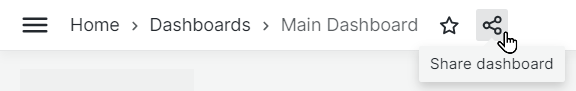
\includegraphics[width=7cm]{../Images/ManualeUtente/Light/toolbar_dettaglio_share.png}}
    \caption{Pulsante "Share"}
    \label{fig:my_label}
\end{figure}

\paragraph{Intervallo temporale}
Il menu a tendina "Intervallo temporale" permette all'utente di selezionare l'intervallo temporale desiderato per la visualizzazione dei dati. La \textit{dashboard}\textsubscript{\textit{G}} offre una serie di intervalli predefiniti e, inoltre, permette all'utente di personalizzarli secondo le proprie necessità. \\
Eventuali aggregazioni delle misurazioni o operazioni effettuate sui dati verranno applicate in base all'intervallo temporale selezionato.
\begin{figure}[H]
    \centering
    \fbox{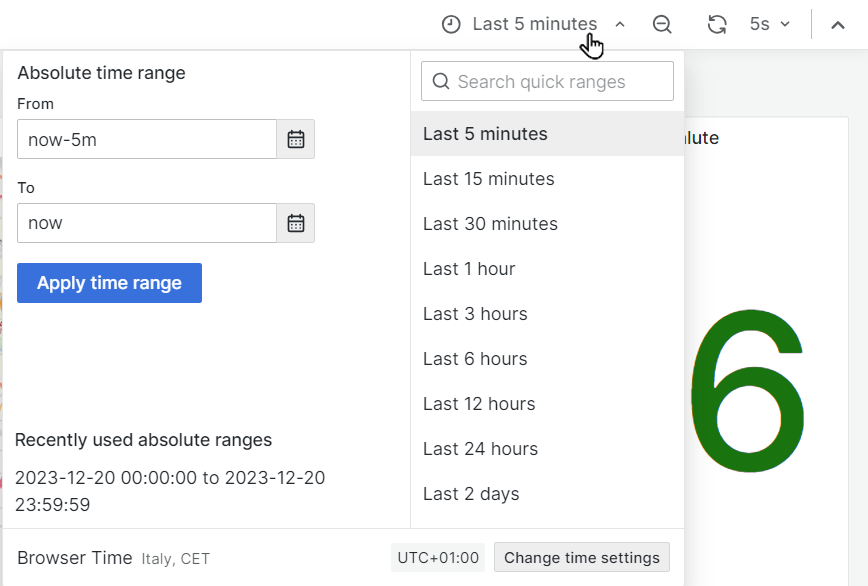
\includegraphics[width=7cm]{../Images/ManualeUtente/Light/toolbar_dettaglio_timerange.png}}
    \caption{Menu "Intervallo temporale"}
    \label{fig:my_label}
\end{figure}

\paragraph{Zoom out}
Il pulsante "Zoom out" consente all'utente di regolare la visualizzazione dei grafici per mostrare un intervallo temporale più ampio, secondo intervalli temporali predefiniti. 
\begin{figure}[H]
    \centering
    \fbox{
\includegraphics[width=7cm]{../Images/ManualeUtente/Light/toolbar_dettaglio_zoomout.png}}
    \caption{Pulsante "Zoom out"}
    \label{fig:my_label}
\end{figure}

\paragraph{Ricarica dashboard}
Il pulsante "Ricarica \textit{dashboard}\textsubscript{\textit{G}}" permette all'utente di aggiornare la \textit{dashboard}\textsubscript{\textit{G}} attuale per visualizzare i dati più recenti.  Inoltre, offre un menu a tendina attraverso il quale l'utente può impostare la frequenza di aggiornamento automatico della \textit{dashboard}\textsubscript{\textit{G}} o disattivarlo, se necessario.  
\begin{figure}[H]
    \centering
    \fbox{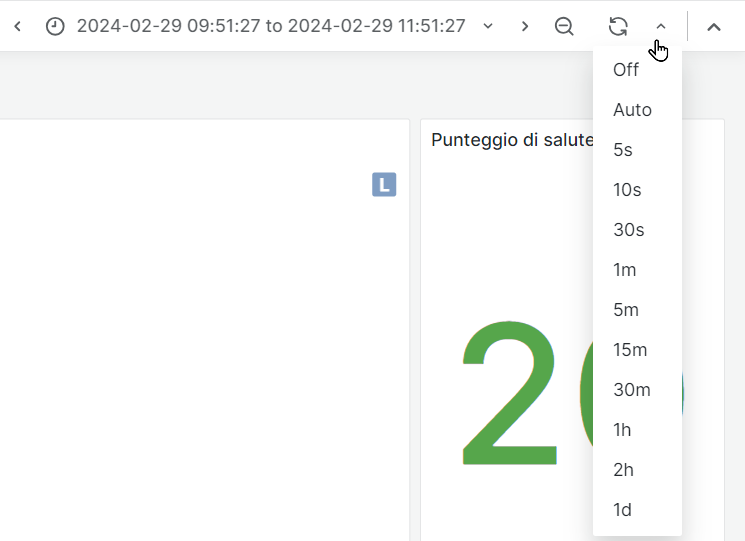
\includegraphics[width=8.5cm]{../Images/ManualeUtente/Light/toolbar_dettaglio_refresh.png}}
    \caption{Pulsante "Ricarica dashboard"}
    \label{fig:my_label}
\end{figure}

\subsubsection{Pannelli}
I pannelli costituiscono la parte principale della \textit{dashboard}\textsubscript{\textit{G}}, mostrando i dati in modo interattivo. Ogni pannello è un \textit{widget}\textsubscript{\textit{G}} progettato per visualizzare un tipo specifico di dati, adottando grafici di diversa natura in base alla tipologia di informazioni. \\
Ogni pannello contiene delle informazioni specifiche del grafico che rappresenta come ad esempio:
\begin{itemize}
    \item il nome pannello;
    \item una breve descrizione del pannello (se presente);
    \item una legenda del grafico (se presente);
    \item un menù a tendina per la selezione delle opzioni del grafico;
    \item visualizzazione dei dati misurati.
\end{itemize}

\paragraph{Descrizione del pannello}
La descrizione del pannello è una breve spiegazione del contenuto del pannello, che può essere visualizzata cliccando sull'icona "i" posta in alto a sinistra del pannello.  
\begin{figure}[H]
    \centering
    \fbox{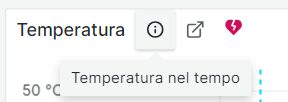
\includegraphics[width=5cm]{../Images/ManualeUtente/Light/descrizione_panel.png}}
    \caption{Descrizione del pannello}
    \label{fig:my_label}
\end{figure}

\paragraph{Legenda del grafico}
La legenda del grafico è una sezione del pannello che mostra la chiave di lettura dei dati visualizzati nel grafico. Questa sezione è utile per comprendere il significato dei colori e delle forme utilizzate nel grafico. \\
Inoltre, tramite la legenda, gli utenti possono interagire direttamente con il grafico. Ad esempio, è possibile isolare le informazioni relative a uno specifico \textit{sensore}\textsubscript{\textit{G}}. Facendo clic sul nome del \textit{sensore}\textsubscript{\textit{G}} d'interesse nella legenda del grafico, gli utenti possono concentrarsi esclusivamente sull'andamento del singolo \textit{sensore}\textsubscript{\textit{G}} selezionato. Per tornare alla visualizzazione originale, è sufficiente cliccare nuovamente sul nome del \textit{sensore}\textsubscript{\textit{G}} nella legenda.
\begin{figure}[H]
    \centering
    \fbox{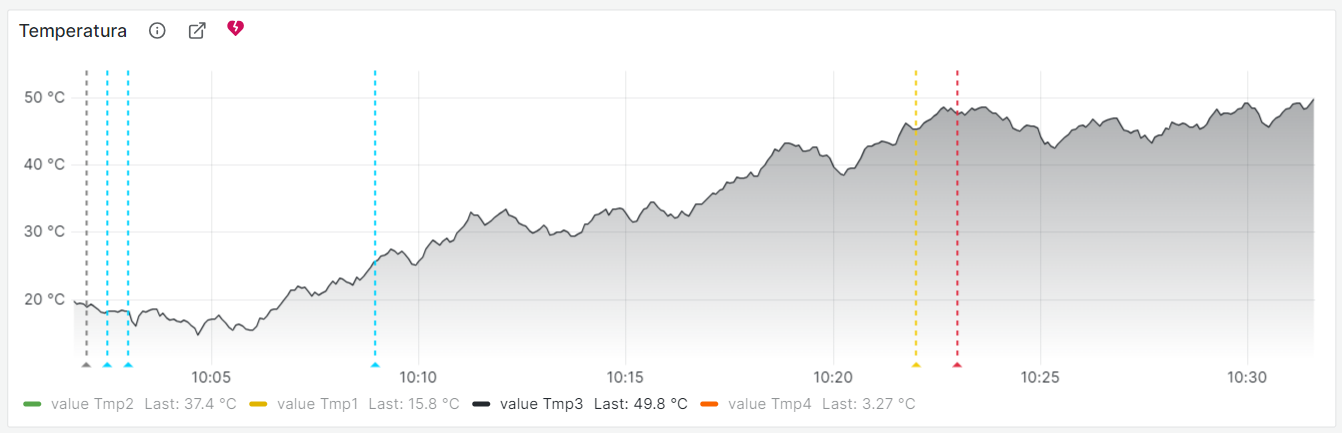
\includegraphics[width=12cm]{../Images/ManualeUtente/Light/panel_singolo_grafico.png}}
    \caption{Visualizzazione del grafico con la misurazione isolata}
    \label{fig:my_label}
\end{figure}
É inoltre possibile cambiare il colore dell'andamento di una misurazione nel grafico cliccando sul colore corrispondente nella legenda.
\begin{figure}[H]
    \centering
    \fbox{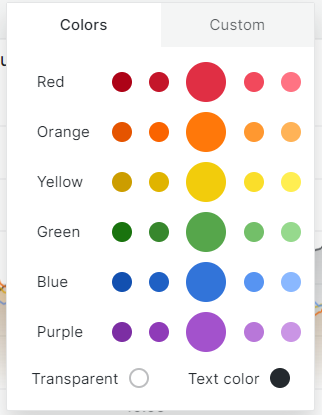
\includegraphics[width=3.5cm]{../Images/ManualeUtente/Light/colori_panel.png}}
    \caption{Cambiare il colore del grafico}
    \label{fig:my_label}
\end{figure}


\paragraph{Opzioni del pannello}
Tramite il menù a tendina delle opzioni del pannello, l'utente può accedere a diverse funzionalità aggiuntive, tra cui:
\begin{itemize}
    \item visualizzare il singolo pannello a schermo intero;
    \item condividere il pannello con altri utenti o esportarlo come file;
    \item ispezionare i dati delle misurazioni del grafico o l'intero pannello in formato \textit{JSON}\textsubscript{\textit{G}};
    \item nascondere o visualizzare la legenda (se presente).
\end{itemize}
\begin{figure}[H]
    \centering
    \fbox{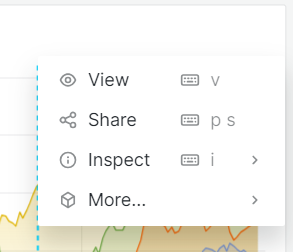
\includegraphics[width=5cm]{../Images/ManualeUtente/Light/panel_options.png}}
    \caption{Opzioni del pannello}
    \label{fig:my_label}
\end{figure}


\subsubsection{Tipologie dei grafici}
\label{subsec:tipologie_grafici}

\paragraph{Mappa sensori}
\hypertarget{par:mappa_sensori}{}
Ogni \textit{sensore}\textsubscript{\textit{G}} rappresentato sulla mappa è identificato da un pin colorato, il quale visualizza la tipologia di \textit{sensore}\textsubscript{\textit{G}} installato mediante un'icona esemplificativa. La colorazione del pin può variare in base alla tipologia di \textit{sensore}\textsubscript{\textit{G}} e alle condizioni della misurazione; ad esempio, per i sensori di rilevamento dei guasti elettrici, il pin potrebbe assumere una colorazione rossa o verde a seconda della situazione.  

Cliccando su un pin, gli utenti possono accedere alle informazioni dettagliate relative al \textit{sensore}\textsubscript{\textit{G}} specifico selezionato.
\begin{figure}[H]
    \centering
    \fbox{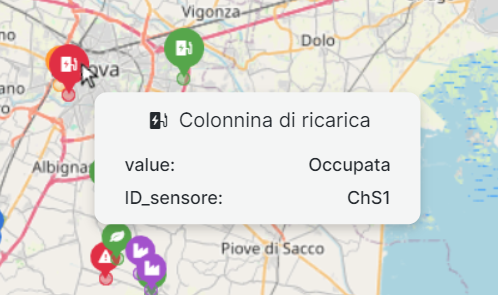
\includegraphics[width=8cm]{../Images/ManualeUtente/Light/dettaglio_mappa_light2.png}}
    \caption{Mappa sensori}
    \label{fig:my_label}
\end{figure}


\paragraph{Grafico a linee}
\hypertarget{par:grafico_linee}{}
I grafici a linee rappresentano l'andamento delle misurazioni ottenute dai sensori nel tempo. Ogni linea del grafico corrisponde a un \textit{sensore}\textsubscript{\textit{G}}, e il suo colore è associato in modo univoco ad un determinato \textit{sensore}\textsubscript{\textit{G}} per favorire una facile distinzione. Se l'utente interagisce con il cursore del mouse sul grafico, potrà visualizzare le informazioni relative alla misurazione di un \textit{sensore}\textsubscript{\textit{G}} specifico nel punto desiderato. Questo punto corrisponderà a un tempo riportato sull'asse delle ascisse.  
\begin{figure}[H]
    \centering
    \fbox{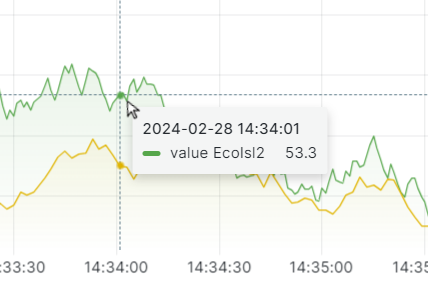
\includegraphics[width=8cm]{../Images/ManualeUtente/Light/dettaglio_time_series_light_bordo.png}}
    \caption{Grafico a linee}
    \label{fig:my_label}
\end{figure}

\paragraph{Lista allerte}
Il pannello contenente la lista degli alert mostra le notifiche delle avvertenze che i sensori hanno riscontrato. Per ciascuna notifica è possibile visualizzare il tipo di avviso, il tempo trascorso dall'attivazione dell'avviso e le istanze coinvolte. \\
Tramite il menu a tendina dedicato a ciascuna notifica, l'utente potrà visualizzare i dettagli dell'avviso.
\begin{figure}[H]
    \centering
    \fbox{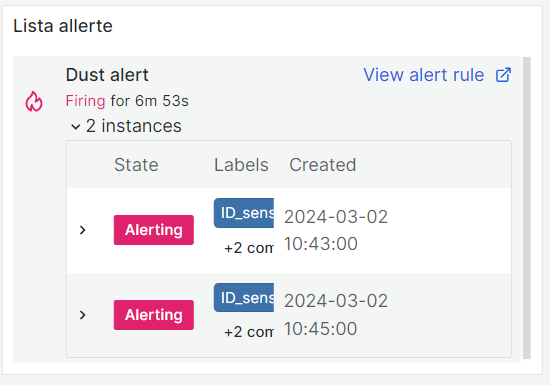
\includegraphics[width=8cm]{../Images/ManualeUtente/Light/alert_panel.png}}
    \caption{Pannello lista allerte}
    \label{fig:my_label}
\end{figure}

\paragraph{Vista tabellare}
\hypertarget{par:tabella}{}
Un grafico tabellare è una rappresentazione visiva dei dati organizzati in forma di tabella, dove le informazioni sono disposte in righe e colonne. Ogni riga della tabella rappresenta una misurazione trasmesse da un \textit{sensore}\textsubscript{\textit{G}}, mentre le colonne rappresentano le diverse variabili o attributi associati. Le celle della tabella possono contenere testo, numeri o altre tipologie di dati, a seconda della natura dei dati rappresentati.
\begin{figure}[H]
    \centering
    \fbox{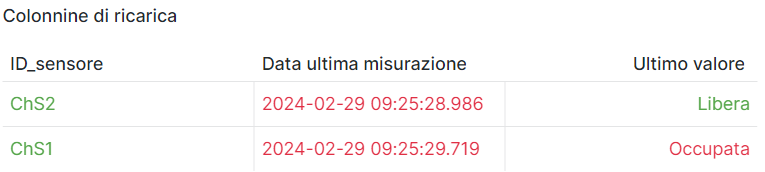
\includegraphics[width=8cm]{../Images/ManualeUtente/Light/vista_tabellare.png}}
    \caption{Vista tabellare}
    \label{fig:my_label}
\end{figure}

\paragraph{Grafico a quadrante}
\hypertarget{par:grafico_quadrante}{}
I grafici a quadrante, noti anche come \textit{gauge}, consentono di visualizzare un singolo valore all'interno di un intervallo specifico. 

\begin{figure}[H]
    \centering
    \fbox{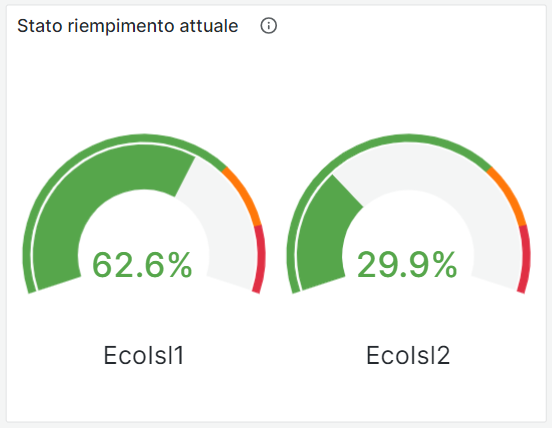
\includegraphics[width=6cm]{../Images/ManualeUtente/Light/gauge_light.png}}
    \caption{Grafico a quadrante}
    \label{fig:my_label}
\end{figure}


\paragraph{Grafico visualizzazione statistiche}
\hypertarget{par:visu_stat}{}
Questa tipologia di grafico consente una visualizzazione chiara e intuitiva dei dati numerici derivati da calcoli e aggregazioni effettuate sulle misurazioni ottenute dai sensori. 
\begin{figure}[H]
    \centering
    \fbox{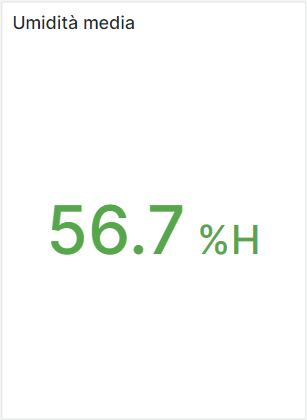
\includegraphics[width=4cm]{../Images/ManualeUtente/Light/stats.png}}
    \caption{Grafico visualizzazione statistiche}
    \label{fig:my_label}
\end{figure}


\subsubsection{Gestione variabili dei grafici}
\hypertarget{par:gestione_variabili_panel}{}
La nostra \textit{piattaforma}\textsubscript{\textit{G}} consente all'utente di gestire di quali sensori visualizzare le misurazioni. Attraverso la selezione delle variabili presenti nella \textit{dashboard}\textsubscript{\textit{G}}, è possibile aggiungere o rimuovere la visualizzazione dei dati relativi ad uno o più sensori, offrendo all'utente la possibilità di personalizzare la propria esperienza di utilizzo. 
\begin{figure}[H]
    \centering
    \fbox{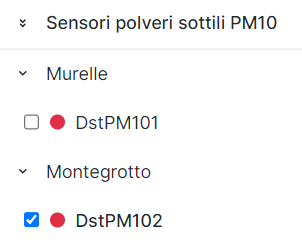
\includegraphics[width=6cm]{../Images/ManualeUtente/Light/variabili_base.png}}
    \caption{Pannello variabili dei grafici}
    \label{fig:my_label}
\end{figure}


\subsection{Gruppi di pannelli in dettaglio}
I gruppi di pannelli sono stati progettati per offrire agli utenti una visione completa e dettagliata di un aspetto specifico della città. Ogni gruppo è composto da una serie di pannelli che collaborano per presentare informazioni relative a una singola categoria di dati, come temperatura, umidità, presenza di polveri sottili e altre metriche pertinenti. 

Questi pannelli sono appositamente configurati per essere interattivi e fornire agli utenti dettagli in risposta alle azioni eseguite.
 \\
\subsubsection{City Manager}
Il gruppo di pannelli "City Manager" è stato appositamente concepito per offrire agli utenti una panoramica dettagliata e completa delle informazioni relative alla città. Questo insieme di pannelli è stato progettato con l'obiettivo di fornire una visione esaustiva e immediata dello stato attuale del contesto urbano. \\
Il gruppo è composto da quattro pannelli principali:
\begin{itemize}
    \item \textbf{Pannello di selezione delle celle}: consente agli utenti di selezionare le variabili inerenti alle celle della città affinché il gruppo di pannelli possa visualizzare le informazioni corrispondenti;
    \item \textbf{Mappa dei sensori}: visualizza la posizione dei sensori desiderati nella città;
    \item \textbf{Punteggio di salute}: visualizza il punteggio di salute della città, generato dal calcolo di un indice di qualità delle misurazioni effettuate dai sensori;
    \item \textbf{Lista delle avvertenze}: visualizza le avvertenze relative alla città. Queste avvertenze sono generate dal \textit{sistema}\textsubscript{\textit{G}} in base alle misurazioni effettuate dai sensori e sono visualizzate in tempo reale.
\end{itemize}
\begin{figure}[H]
    \centering
    \fbox{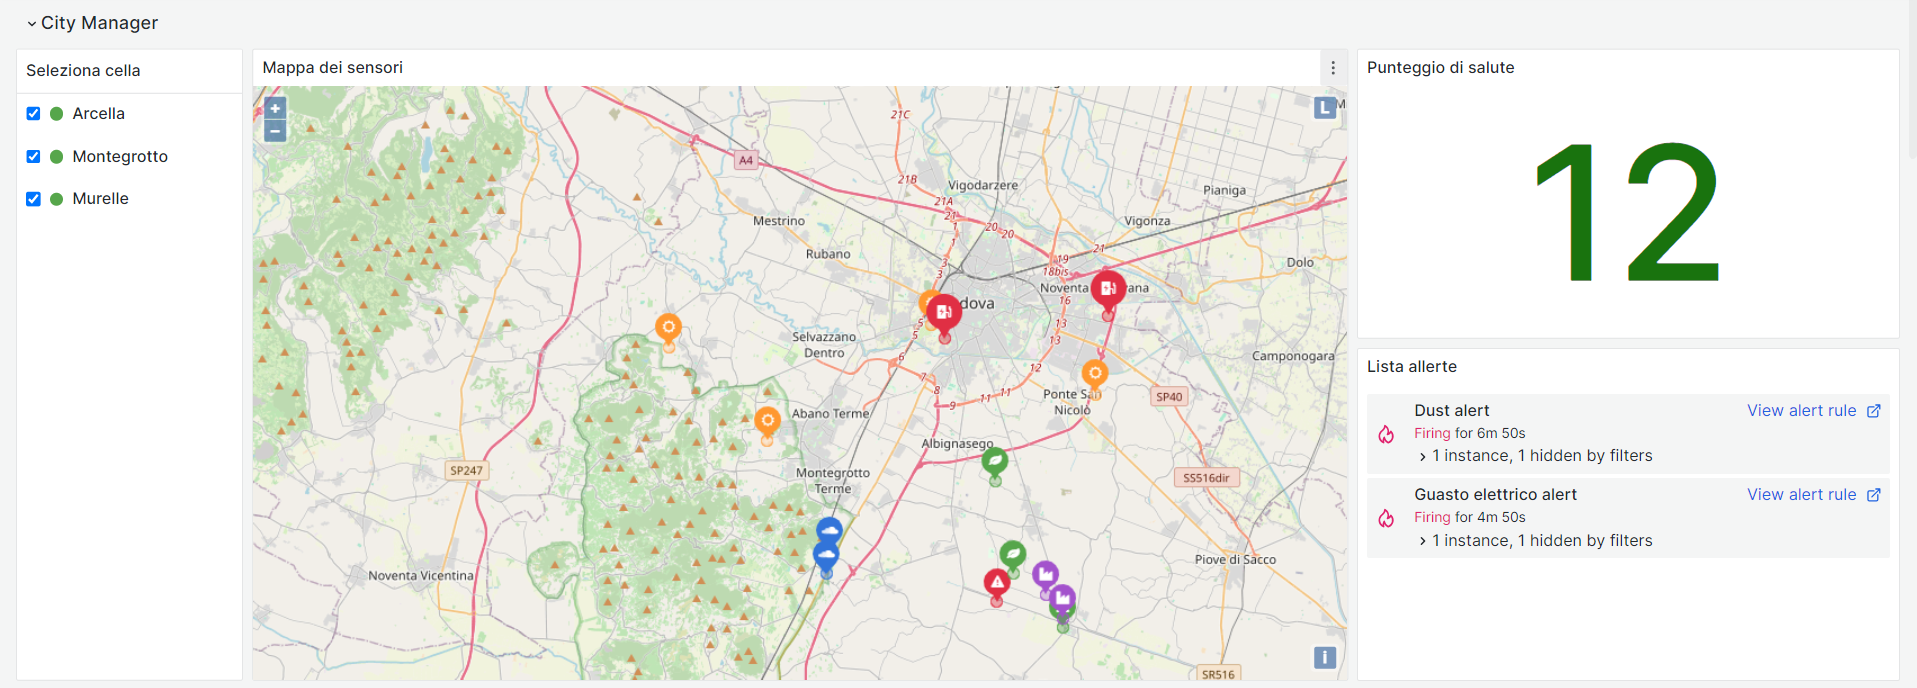
\includegraphics[width=15cm]{../Images/ManualeUtente/Light/gruppo_pannelli_city_manager.png}}
    \caption{Gruppo di pannelli "City Manager"}
    \label{fig:my_label}
\end{figure} 


\subsubsection{Temperatura, Umidità, Polveri sottili}
I gruppi di pannelli "Temperatura", "Umidità" e "Polveri sottili" hanno una struttura simile. Per facilità di comprensione, verrà descritto solo il gruppo di pannelli "Temperatura" ma le stesse informazioni si applicano anche agli altri due gruppi. \\ 
Il gruppo di pannelli "Temperatura" è composto da tre pannelli:
\begin{itemize}
    \item \textbf{Pannello di selezione dei sensori}: consente agli utenti di selezionare i sensori desiderati affinché il gruppo di pannelli possa visualizzare le informazioni corrispondenti;
    \item \textbf{Grafico a linee}: visualizza la temperatura rilevata dai sensori selezionati tramite un grafico a linee descritto nel paragrafo  ~\hyperlink{par:grafico_linee}{\S 3.2.3 - Grafico a linee};
    \item \textbf{Temperatura media}: visualizza la temperatura media rilevata dai sensori selezionati in un determinato intervallo di tempo. La temperatura media viene mostrata all'utente attraverso un grafico "visualizzazione statistiche" come descritto nel paragrafo ~\hyperlink{par:visu_stat}{\S 3.2.3 - Grafico visualizzazione statistiche} e attraverso un valore numerico.
\end{itemize}
\begin{figure}[H]
    \centering
    \fbox{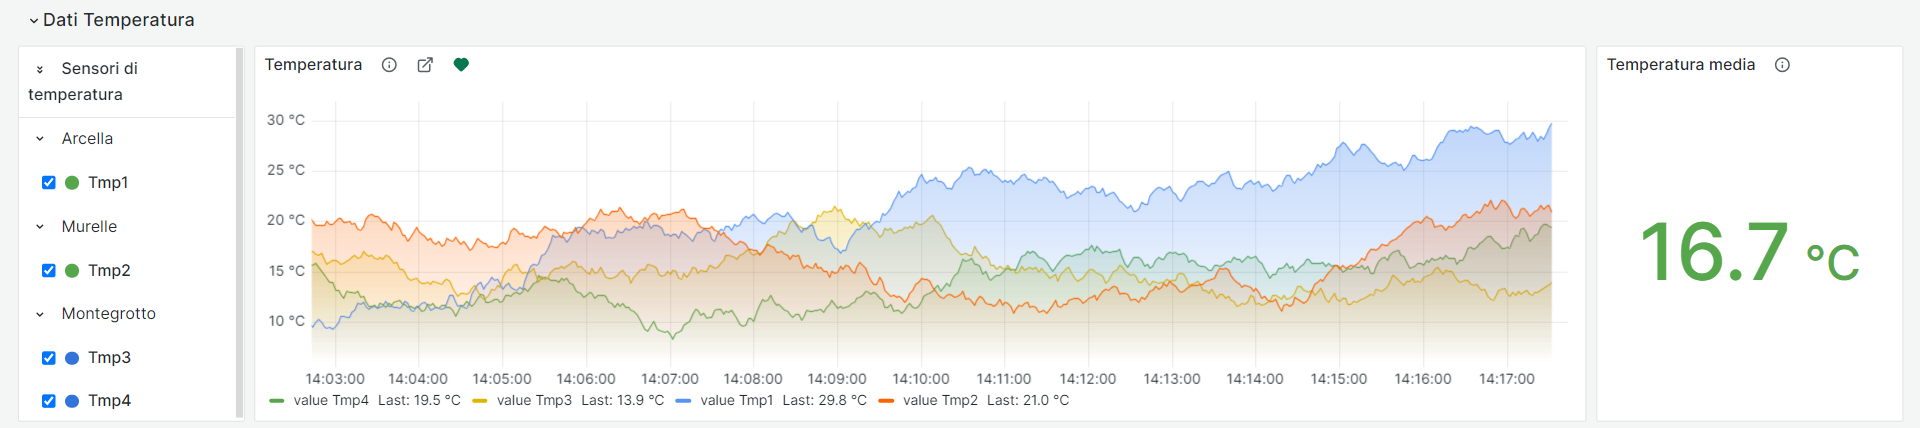
\includegraphics[width=15cm]{../Images/ManualeUtente/Light/gruppo_pannelli_temperatura.png}}
    \caption{Gruppo di pannelli "Temperatura"}
    \label{fig:my_label}
\end{figure}

\subsubsection{Isole ecologiche}
Il gruppo di pannelli "Isole ecologiche" è stato progettato per fornire una visione completa delle informazioni relative alle isole ecologiche. \\
Questo gruppo di pannelli differisce dagli altri descritti sopra in quanto al posto della visualizzazione della temperatura media è presente un grafico a quadrante come descritto nel paragrafo ~\hyperlink{par:grafico_quadrante}{\S 3.2.3 - Grafico a quadrante} che visualizza la percentuale di riempimento delle isole ecologiche. \\
\begin{figure}[H]
    \centering
    \fbox{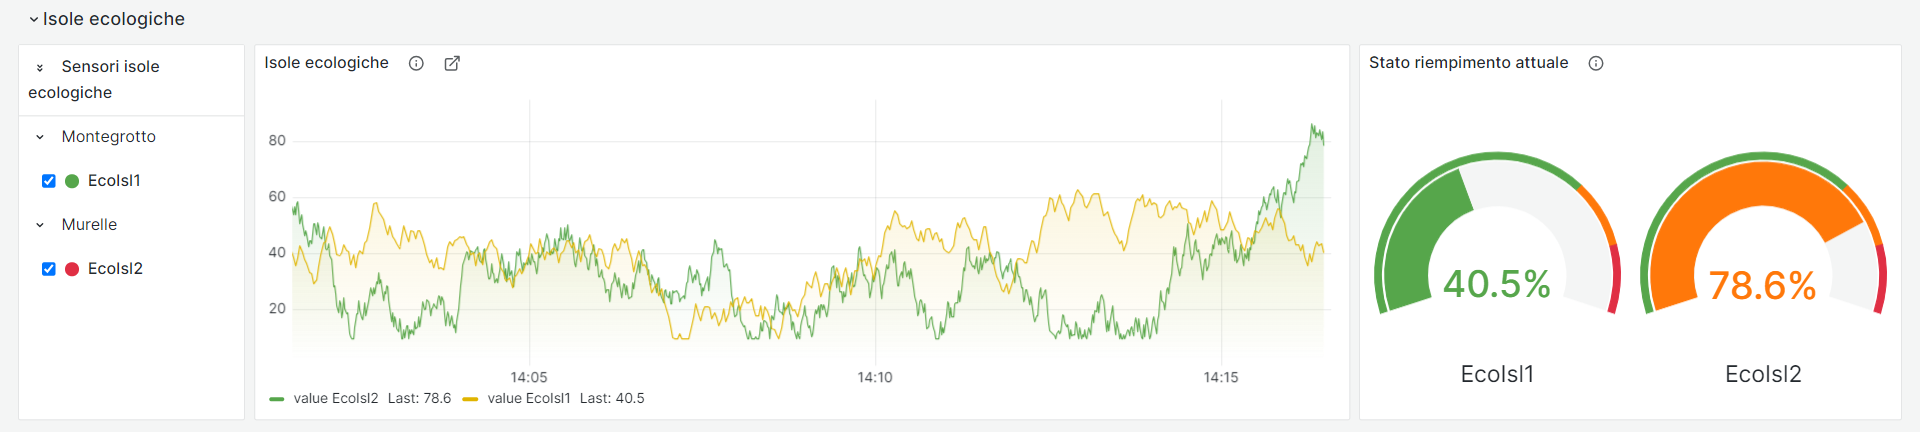
\includegraphics[width=15cm]{../Images/ManualeUtente/Light/gruppo_pannelli_isole.png}}
    \caption{Gruppo di pannelli "Isole ecologiche"}
    \label{fig:my_label}
\end{figure}


\subsubsection{Presenza acqua, Colonnine di ricarica, Guasti elettrici}
I gruppi di pannelli "Presenza acqua", "Colonnine di ricarica" e "Guasti elettrici" hanno una struttura simile. Per facilità di comprensione, verrà descritto solo il gruppo di pannelli "Presenza acqua" ma le stesse informazioni si applicano anche agli altri due gruppi. \\
Il gruppo "Presenza acqua" è composto da quattro pannelli:
\begin{itemize}
    \item \textbf{Sensori presenza acqua}: consente agli utenti di selezionare le variabili (descritte in dettaglio nella sezione ~\hyperlink{par:gestione_variabili_panel}{\S3.2.4}) relative ai sensori desiderati affinché il gruppo di pannelli possa visualizzare le informazioni corrispondenti;
    \item \textbf{Sensori di soglia non attivi}: visualizza i sensori di soglia non attivi tramite un pannello di tipo "visualizzazione statistiche" come descritto nel paragrafo ~\hyperlink{par:visu_stat}{\S 3.2.3 - Grafico visualizzazione statistiche};
    \item \textbf{Sensori di soglia attivi}: visualizza i sensori di soglia attivi tramite un pannello di tipo "visualizzazione statistiche" come descritto nel paragrafo ~\hyperlink{par:visu_stat}{\S 3.2.3 - Grafico visualizzazione statistiche};
    \item \textbf{Sensori di livello acqua}: visualizza i sensori di livello dell'acqua in tabella tramite un pannello di tipo "vista tabellare" come descritto nel paragrafo ~\hyperlink{par:tabella}{\S3.2.3 - Vista tabellare}.
\end{itemize}
\begin{figure}[H]
    \centering
    \fbox{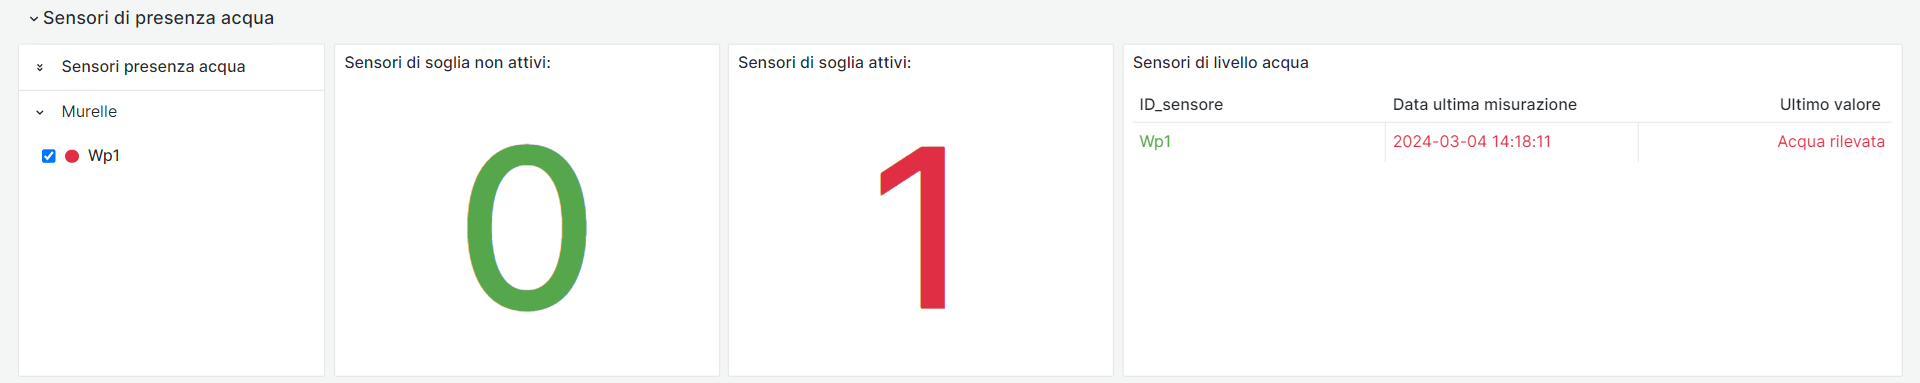
\includegraphics[width=15cm]{../Images/ManualeUtente/Light/gruppo_pannelli_presenza_acqua.png}}
    \caption{Gruppo di pannelli "Presenza acqua"}
    \label{fig:my_label}
\end{figure}

\subsubsection{Minimizzare e massimizzare i gruppi di pannelli}
Ogni gruppo di pannelli può essere minimizzato o massimizzato. Per minimizzare un gruppo di pannelli, l'utente deve fare clic sul nome del gruppo di pannelli o sulla freccetta posta vicino a esso. Per tornare alla visualizzazione massimizzata, l'utente deve fare nuovamente clic sul nome del gruppo di pannelli o sulla freccetta. \\
\begin{figure}[H]
    \centering
    \fbox{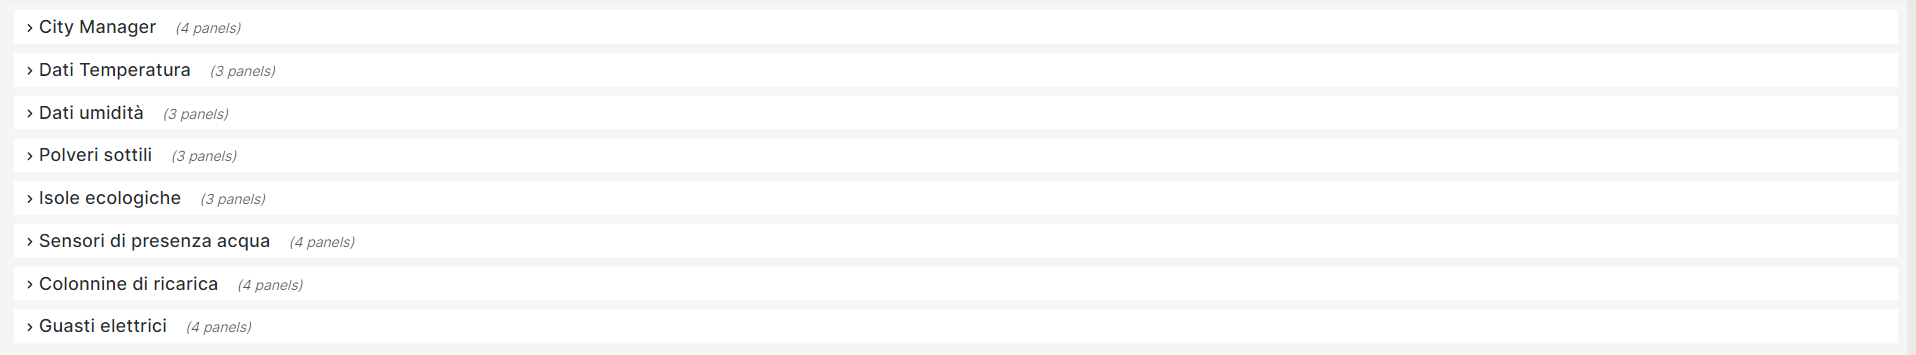
\includegraphics[width=13cm]{../Images/ManualeUtente/Light/gruppo_pannelli_chiusi.png}}
    \caption{Gruppo di pannelli minimizzati}
    \label{fig:my_label}
\end{figure}



\subsection{Dashboard dettagliate}
\subsubsection{Accesso alle dashboard dettagliate}
Cliccando su un bottone posto in ciascun grafico a linee nei gruppi di pannelli, l'utente verrà reindirizzato in una \textit{dashboard}\textsubscript{\textit{G}} contenente i dettagli relativi al gruppo selezionato. 
\begin{figure}[H]
    \centering
    \fbox{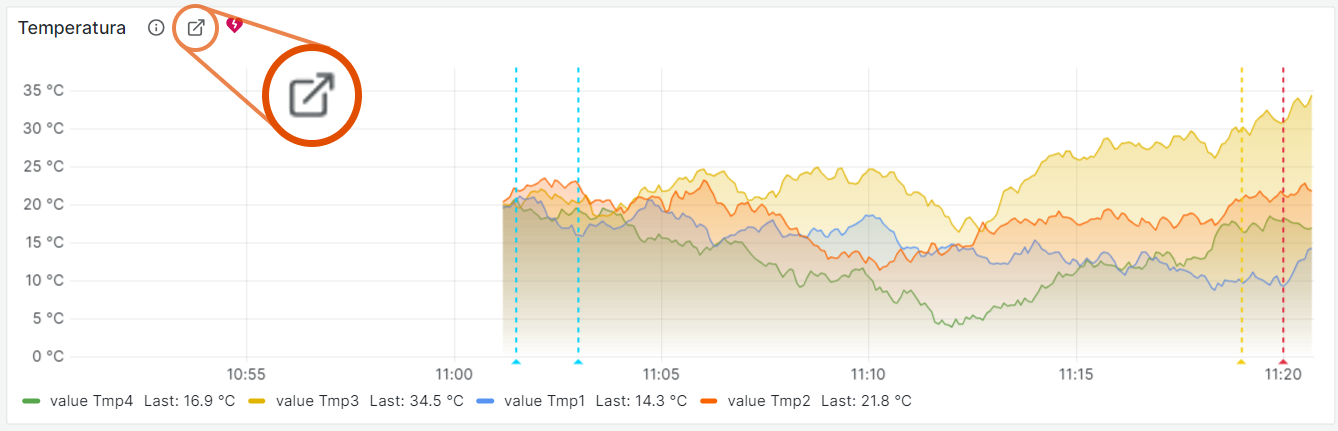
\includegraphics[width=15cm]{../Images/ManualeUtente/Light/temperature_graph_dashboard_dettaglio_alert.png}}
    \caption{Accesso alle dashboard dettagliate}
    \label{fig:my_label}
\end{figure}

\subsubsection{Zoom in Dashboard}
La \textit{dashboard}\textsubscript{\textit{G}} "Zoom in \textit{Dashboard}\textsubscript{\textit{G}}" rappresenta il cruscotto verso cui gli utenti sono reindirizzati dopo aver cliccato su un bottone di un gruppo di pannelli. Questa \textit{dashboard}\textsubscript{\textit{G}} è progettata per mostrare in dettaglio le informazioni relative al gruppo di pannelli selezionato, adattando le \textit{query}\textsubscript{\textit{G}} dei vari pannelli per visualizzare esclusivamente i dati pertinenti al gruppo scelto. 
\begin{figure}[H]
    \centering
    \fbox{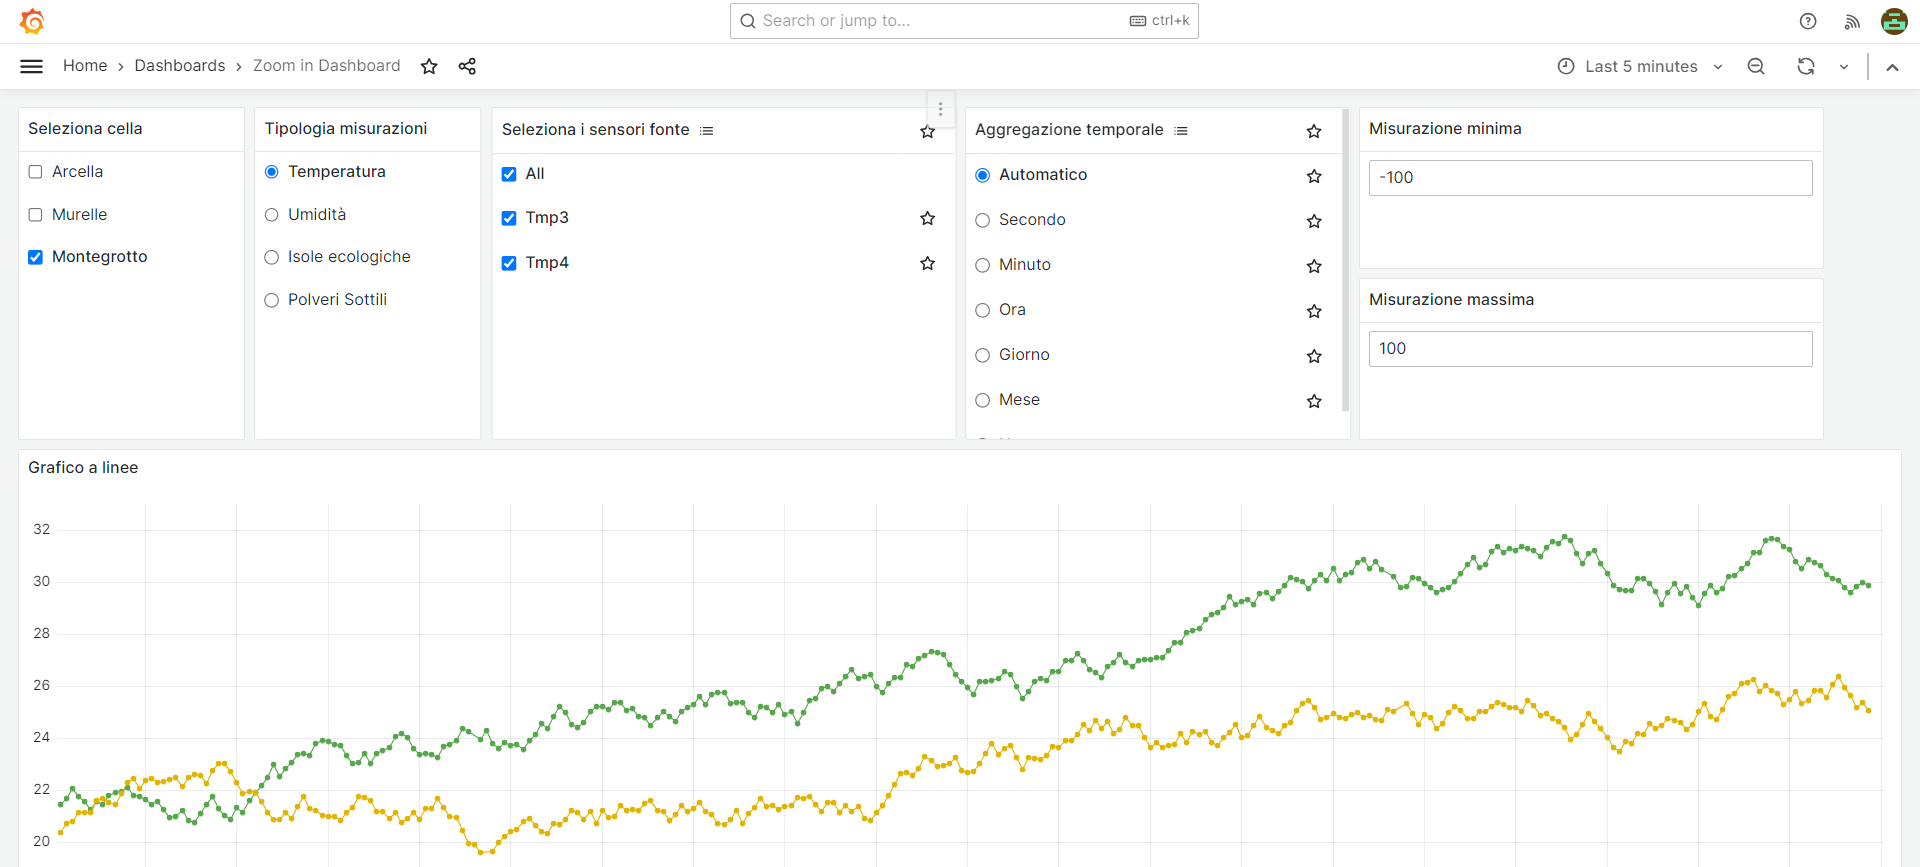
\includegraphics[width=15cm]{../Images/ManualeUtente/Light/dashboard_zoom_in.png}}
    \caption{Dashboard "Zoom in Dashboard"}
    \label{fig:my_label}
\end{figure}

\paragraph{Variabili di ricerca}

La \textit{dashboard}\textsubscript{\textit{G}} "Zoom in \textit{Dashboard}\textsubscript{\textit{G}}" offre all'utente la possibilità di personalizzare la visualizzazione dei dati attraverso la modifica dinamica delle variabili di ricerca. Questa flessibilità consente agli utenti di adattare le \textit{query}\textsubscript{\textit{G}} dei grafici in tempo reale alle loro specifiche esigenze, selezionando e visualizzando solo i dati pertinenti.\\
Le variabili offriranno la possibilità di visualizzare i dati in base a diversi parametri, tra cui:
\begin{itemize}
    \item le suddivisioni territoriali delle città;
    \item le tipologie specifiche dei sensori;
    \item il codice univoco attribuito ai singoli sensori;
    \item le diverse aggregazioni temporali applicate ai dati;
    \item il valore massimo e il valore minimo che una misurazione può assumere.
\end{itemize}
\begin{figure}[H]
    \centering
    \fbox{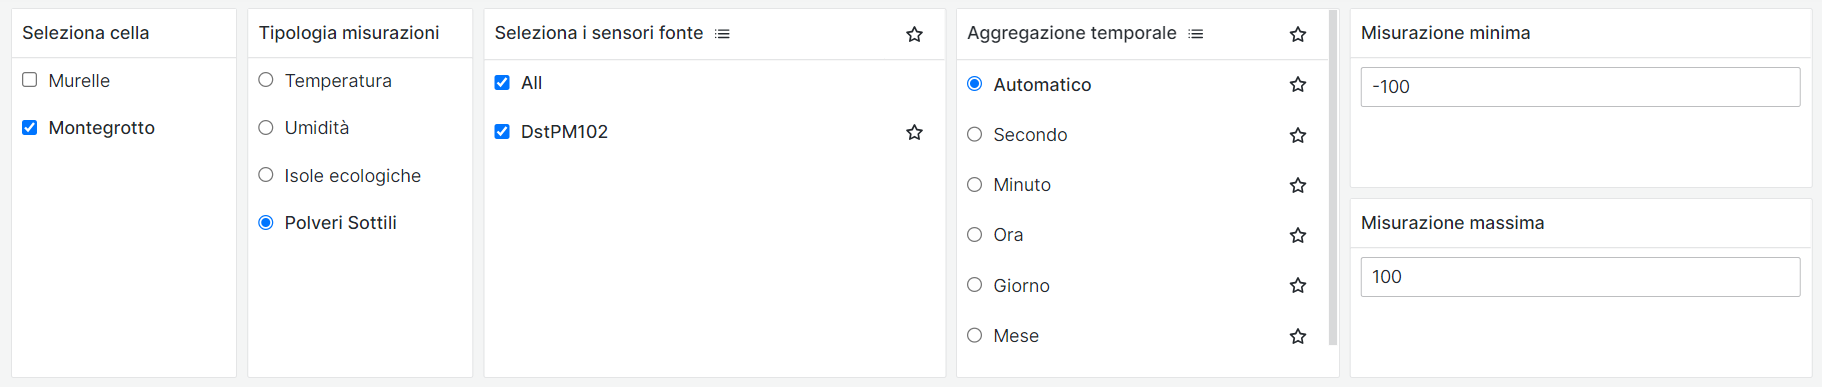
\includegraphics[width=15cm]{../Images/ManualeUtente/Light/variabili_dettaglio_zoom_in.png}}
    \caption{Variabili di ricerca}
    \label{fig:my_label}
\end{figure}



